\subsection{Climbing robots}\label{sota_climbers}
Climbing robots are systems capable of supporting its own weight against
gravity, moving in simple or complex geometric structures, such as
walls, ceilings and roofs, turbine blades and nuclear plants.
Climbers provide operational efficiency in hazardous environments, and increase
operators health and safety. Some applications for climbing robots are:
skyscrapers inspection and cleaning, nuclear power
plants storage tanks diagnosis, shell ships and turbines welding and
maintenance\citep{armada2003application}.
%Robôs escaladores são sistemas capazes de sustentar seu próprio peso contra a
%gravidade, movendo-se em simples ou complexas estruturas geométricas, como
%paredes, tetos e telhados, palhetas de turbinas e plantas nucleares.
%Essa classe de robôs oferece eficiência operacional em ambientes
%de alta periculosidade, sendo utilizados visando saúde e segurança dos
%trabalhadores, como em inspeção e limpeza de arranha-céus, diagnóstico de
%tanques de armazenamento em plantas nucleares, solda e manutenção de cascos de
%navios e palhetas de turbinas \citep{armada2003application}. 

The major challenges in climbers system designs are mobility and
adhesion, power consumption, load capacity and weight. In
\cite{modular} and \cite{climbsurv}, climbers are divided into types of
locomotive mechanisms: legs; walker; translation; wheels; tracks;
advance by arms; cable-driven; and biomimetics. And adhesion types:
suction or pneumatic; magnetic; electrostatic; chemistry; gripping; and hybrid.
%Os grandes desafios nos projetos de sistemas escaladores são mobilidade e
%aderência, além de consumo de energia, capacidade de carga e peso. Em
%\cite{modular} e \cite{climbsurv}, os robôs escaladores são divididos em tipos
%de locomoção:
%pernas; como andador; utilizando segmentos deslizantes; rodas; esteiras; avanço
%pendurado por braços; por cabos; e biomimética. E categorias de adesão: sucção
%ou pneumática; magnética; eletrostática; química; preensão; e híbrida.

In the specific case of the HVOF coating problem in hydropower turbines, the
following climber robots should be investigated:
%No caso específico deste estudo da arte, destacam-se os robôs escaladores com
% as seguintes aplicações:

\begin{itemize}
  \item \emph {ships and turbines}: RRX3 for welding
   \citep{rrx3}, \emph{Climbing Robot for Grit Blasting for cleaning}
   \citep{crgb} and ICM Robot for inspection \citep{icm};
  \item \emph{Industrial}: ROME II \citep{roma} and roma
   CROMSCI \citep{CROMSCI}, both for inspection;
  \item \emph{petrochemical plant}: TRIPILLAR \citep{tripillar} for inspection.
\end{itemize}

The RRX3 (figure~\ref{rrx3}), Daewoo Shipbuilding \& Marine Engineering, is a
robot for hull ship welding. Its adhesion is gripping type, and translation
locomotion type  (sliding segments) and longitudinal locomotion by wheels.
The RRX3 robot has a 1.5 m manipulator with three prismatic joints and three
revolution joints  (3P3R) for welding operation.
%O RRX3 (figura~\ref{rrx3}), Daewoo Shipbuilding and Marine Engineering, é um
%robô para a soldagem de casco de navios. Possui adesão por preensão, locomoção
% transversal utilizando segmentos deslizantes e locomoção longitudinal por rodas. Possui um manipulador de 1.5 m com três juntas
%prismáticas e três juntas de revolução (3P3R) para a operação de soldagem. 

RRX 3 main characteristics are: base and manipulator with
120 kg and 5 kg of payload, respectively; accurately
millimeter manipulator and low speed end effector; robustness; welding tool
operation; limited translation type locomotion.
%As características principais do robô são: base e manipulador com
%capacidades de carga de 120 kg e 5 kg, respectivamente; manipulador com
% precisão milimétrica e efetuador de baixa velocidade; robustez para operar em ambiente de
%alta periculosidade; opera instrumento de solda; e locomoção transversal é
%restrita à aplicação.

\begin{figure}[ht]
\centering
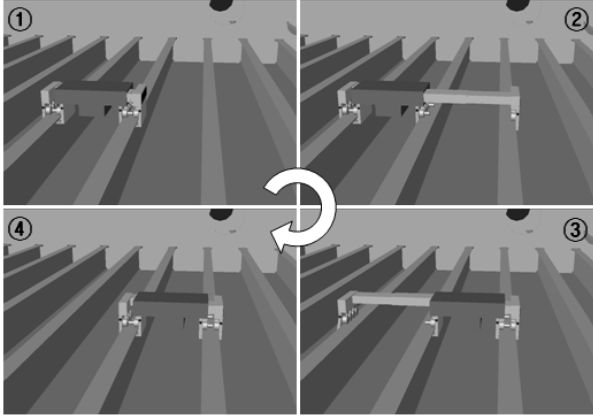
\includegraphics[width=8.4cm]{figs/climbers/RRX3_moving.jpg}
\caption{RRX3 translation locomotion.}
\label{rrx3}
\end{figure}

The \emph{Climbing robot for Grit Blasting} (figura~\ref{grit}), University of
Coruna, is a robot for ship abrasive blasting. The robot moves by two
sliding platforms with magnetic adhesion. The platforms have relative motion
between them and can rotate to compensate ship's hull curvatures or
deflecting of objects.
%O \emph{Climbing robot for Grit Blasting} (figura~\ref{grit}), University of
%Coruna, é um robô para jateamento abrasivo em navios. O robô utiliza duas
% plataformas deslizantes com sistema de adesão por ímã magnético. Os módulos apresentam movimentação relativa entre si e pode rotar
%para compensar as curvaturas do casco do navio ou desviar de objetos. 

The \emph{Climbing robot for Grit Blasting} main characteristics are:
abrasive system similar with HVOF; accurately
millimeter movement; locomotion not applicable to complex structures; no
manipulator.
%As características principais do robô são: base com
%capacidade de carga de sistema abrasivo semelhante a HVOF; base com
%locomoção de precisão milimétrica; locomoção ampla, mas não aplicável a
%estruturas complexas; e não possui manipulador, sendo necessário percorrer todo
%o casco.

\begin{figure}[ht]
\centering
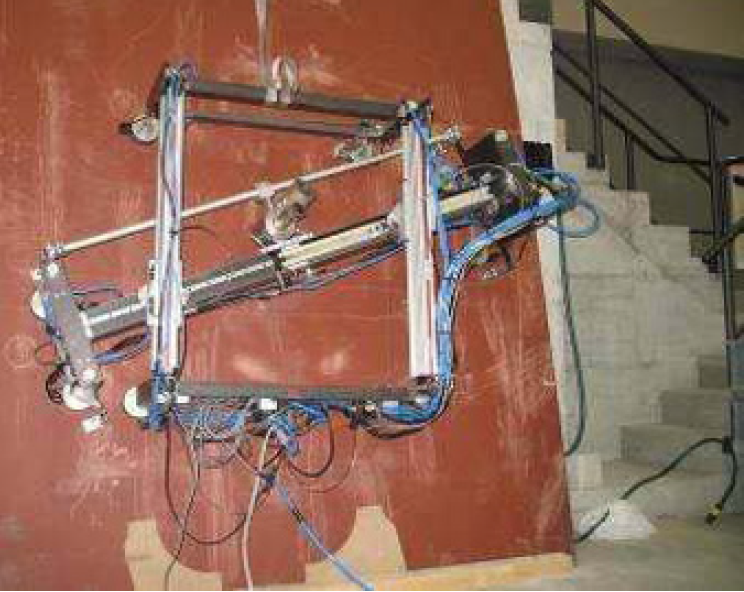
\includegraphics[width=8.4cm]{figs/climbers/grit.png}
\caption{Climbing robot for Grit Blasting}
\label{grit}
\end{figure}


\emph{The Climber} (figure~\ref{icm}), ICM Robotics, is an inspection robot for
wind turbines, coating removal, surface cleaning and coating application.
It has pneumatic adhesion and locomotion by tracks.
%\emph{The Climber} (figura~\ref{icm}), ICM Robotics, é um robô para inspeção de
%turbinas eólicas, remoção de revestimento, limpeza de superfície, e aplicação
% de revestimento.
%Possui adesão pneumática (sucção) e locomoção por esteiras. 

\emph{The Climber} main characteristics are: 25 kg base payload; accurately
millimeter movement; a modular manipulator can be attached to the base; small
size manipulator and low speed; locomotion type presents restriction to
some curvatures.
%As características principais do robô são: base com capacidade de carga de 25
%kg; base com locomoção de precisão milimétrica; manipulador modular pode ser
%acoplado à base; manipulador de dimensão reduzida e baixa velocidade; e
%locomoção apresenta restrição a algumas curvaturas acentuadas.

\begin{figure}[ht]
\centering
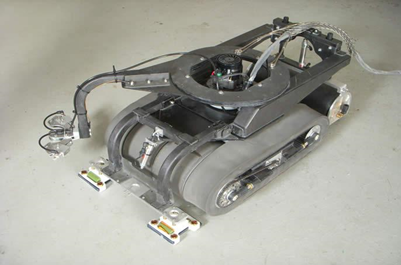
\includegraphics[width=8.4cm]{figs/climbers/icm.png}
\caption{The Climber}
\label{icm}
\end{figure}

The Rome II (figura~\ref{roma2}), University Charles II of Madrid, is an
inspection robot for complex environments. It has pneumatic adhesion and moves
like a caterpillar (biomimicry). Rotation and planning trajectory are performed
optimally to ensure stability and obstacle avoidance.
%O ROMA II (figura~\ref{roma2}), Universidade Carlos II de Madrid, é um robô
% para inspeção de ambientes complexos. A sua tecnologia de adesão é pneumática (sucção) e
%locomove-se como uma lagarta (biomimética). Sua movimentação e planejamento de
%trajetória são realizados de maneira ótima de forma a garantir estabilidade e
%evitar obstáculos. 

The Rome II main characteristics are: high payload capacity; accurately
millimeter movement; no manipulator; locomotion for complex environments.
%As características principais do robô são: base com grande capacidade de carga;
%base com locomoção de precisão milimétrica; não possui manipulador; locomoção
% em ambientes de grande complexidade.

\begin{figure}[ht]
\centering
%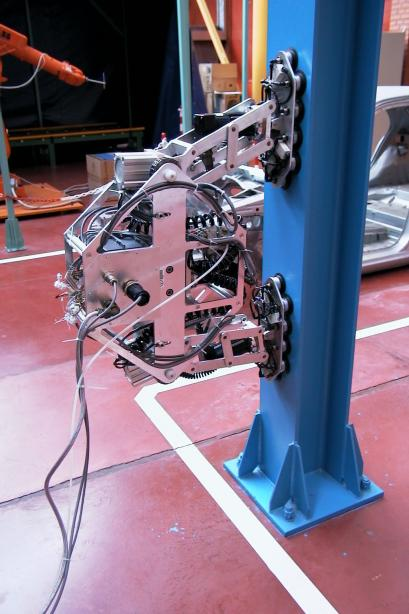
\includegraphics[width=8.4cm]{figs/climbers/roma2.jpg}
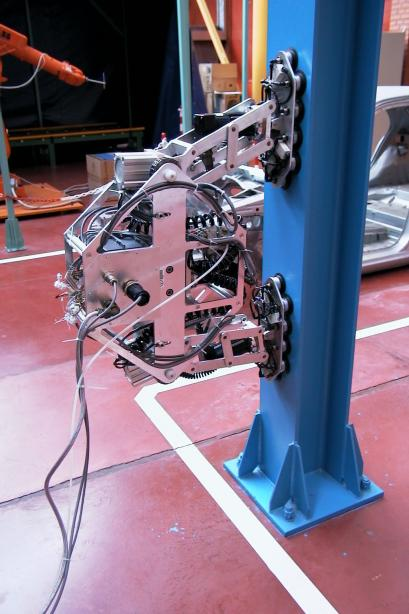
\includegraphics[width=4.2cm,height=4.2cm]{figs/climbers/roma2.jpg}
\caption{ROMA II.}
\label{roma2}
\end{figure}


CROMSCI (figure~\ref{cromsci}), Kaiserslautern University of Technology, is an
inspection and autonomous robot of large concrete walls, as
pillars of bridges and dams. Its adhesion system is seven vacuum
chambers (suction), and valves and pressure sensors for system control. The
locomotion system has omnidirectional wheels.
%CROMSCI (figura~\ref{cromsci}), Kaiserslautern University of Technology, é um
%robô autônomo para inspeção de grandes paredes de concreto, como pilares de
% pontes, barragens. Seu sistema de adesão é composto por sete câmaras de vácuo (sucção), com um sistema
%de controle por válvulas e sensores de pressão para reagir rapidamaente a
%condições adversas. Locomove-se com rodas omnidirecionais para locomoção.

The CROMSCI main characteristics are: low payload capacity; accurately
millimeter movement; no manipulator; low speed.
%As características principais do robô são:
%base com pouca capacidade de carga; base com locomoção de precisão milimétrica;
% não possui manipulador; e apresenta baixa velocidade.

\begin{figure}[ht]
\centering
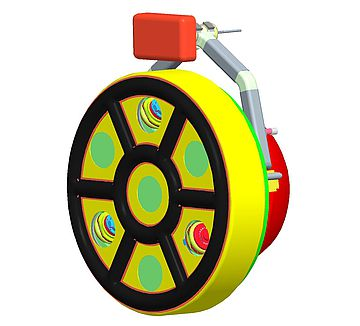
\includegraphics[width=8.4cm]{figs/climbers/cromsci.jpg}
\caption{The CROMSCI robot.}
\label{cromsci}
\end{figure}

TRIPILLAR (figure~\ref{tripillar}), École polytechnique fédérale de Lausanne, is
a small inpection robot (96 x 46 x 64 mm) for petrochemical plants. Its
adhesion is by magnetic legs on a caterpillar triangular shape, and moves by
tracks.
%TRIPILLAR (figura~\ref{tripillar}), École polytechnique fédérale de Lausanne, é
%um robô escalador de pequeno porte (96 x 46 x 64 mm) desenvolvido para a
% inspeção de plantas petroquímicas. Utiliza um sistema como pernas de lagarta magnéticas em um
%formato triangular. Locomove-se por esteiras.

The TRIPILLAR main characteristics are: low payload capacity; accurately
millimeter movement; robust system and application in hazardous environments;
simple control system; small robot; no manipulator; not tested in complex
geometrical structures.
%As características principais do robô são: base com pouca capacidade de
%carga; base com locomoção de precisão milimétrica; sistema robusto a aplicações
%em ambientes de alta periculosidade; sistema de controle simples; robô de
%pequenas dimensões; não possui manipulador; sistema ainda não testado em
% estruturas geométricas complexas.


\begin{figure}[ht]
\centering
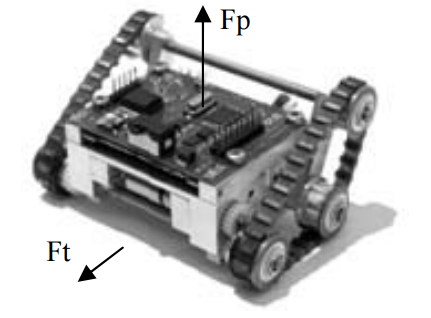
\includegraphics[width=8.4cm]{figs/climbers/tripillar.png}
\caption{TRIPILLAR robot.}
\label{tripillar}
\end{figure}

Climbing robots are widely applicable, have different adhesion solutions and
mobility. There is not, so far, a climber that fulfills all the HVOF
requirements for the turbine blade coating, but some of the systems, such as
\emph{The Climber} (ICM Robotic), can generate complete solutions with
adaptations.
%Os robôs escaladores são utilizados em diversas aplicações e possuem diferentes
%soluções de aderência e locomoção, como foi exposto nesta subseção. Não há,
%até o momento, um robô escalador que possui todas as características
%exigidas para a tarefa de HVOF em pás de turbinas, porém a adaptação de
%alguns desses sistemas, como \emph{The Climber} da ICM Robotic, pode gerar
%soluções completas.

The advantages and disadvantages for climbing robot solution are:
%As vantagens e desvantagens para solução de robôs escaladores são:

\textbf{Advantages:}
\begin{itemize}
  \item Easily installation;
  \item Small size manipulator, since robot moves on blade;
  \item Small base;
  \item Small weight;
  \item Autonomy while operating; 
\end{itemize}

\textbf{Disadvantages:}
\begin{itemize}
  \item Complex locomotion system with obstacle avoidance and path
  planning;
  \item Complex mechanics, as robot should be able to support its weight plus
  the manipulator and the HVOF spary gun;
  \item Robot must be manually installed on each blade or a complex locomotion
  system by arms should be developed;;
  \item Robot safety system must be well developed;
  \item Limited battery or umbilical management system for mobile robots;
\end{itemize}